\documentclass[12pt]{article}
\usepackage[utf8]{inputenc}
\usepackage{float}
\usepackage{amsmath}
\usepackage{amssymb}
\usepackage{tikz}
\usepackage{verbatim}

\usepackage[hmargin=3cm,vmargin=6.0cm]{geometry}
%\topmargin=0cm
\topmargin=-2cm
\addtolength{\textheight}{6.5cm}
\addtolength{\textwidth}{2.0cm}
%\setlength{\leftmargin}{-5cm}
\setlength{\oddsidemargin}{0.0cm}
\setlength{\evensidemargin}{0.0cm}

%misc libraries goes here



\begin{document}


\section*{Student Information } 
%Write your full name and id number between the colon and newline
%Put one empty space character after colon and before newline
Full Name :  mergen\\

% Write your answers below the section tags
\section*{Answer 1}
\textbf{a)} \text{For every 1 to be followed immediately by a 0, length l of the string must be greater than or }\\
\text{equal to 2. When l=2, there is only 1 bit string that 1 followed immediately by 0, such that a$_2$=1.}\\
\text{When l=3, there are 2 bit strings that every 1 followed immediately by 0, such that a$_3$=2.}\\
\text{When l=4, there are 4 bit strings that every 1 followed immediately by 0, such that a$_4$=4.}\\
\text{When l=5, there are 7 bit strings that every 1 followed immediately by 0, such that a$_5$=7.}\\
\text{When l=6, there are 12 bit strings that every 1 followed immediately by 0, such that a$_6$=12.}\\
\text{When l=7, there are 20 bit strings that every 1 followed immediately by 0, such that a$_7$=20.}\\
\text{And so on.It is now clear that we have a recurrence relation with the variable l, length of the bit}\\
\text{string, such that a$_{l}$ = a$_{l-1}$ + a$_{l-2}$ +1; with initial conditions a$_2$=1, and  a$_3$=2.}\\
\vspace*{0.2cm}\\
When we plug in l=9 to the recurrence relation:\\
a$_9$ = a$_8$ + a$_7$ + 1 = ( a$_7$ + a$_6$ + 1) +  (a$_6$ + a$_5$ + 1) + 1 = (20 + 12 + 1) + (12 + 7 + 1) + 1\\
\hspace*{10.2cm} = 33 + 20 + 1 = 54\\
\vspace*{0.4cm}\\
\textbf{b)} Since the arrangement does not constrained the solution, we use combinations of 10 from 8 to 10. \\
\[\sum_{n=8}^{10} C(10,n) = C(10,8) + C(10,9) + C(10,10)\]\\
\hspace*{6.8cm} =  45 + 10 + 1 = 56\\
\vspace*{0.4cm}\\
\textbf{c)} From the theorem at page 561 from the textbook.\\
\[3^{4} - \binom{3}{2}\cdot2^{4} + \binom{3}{1}\cdot1^{4} = 81 - 3\cdot16 - 3\cdot1 = 36\]\\
\vspace*{0.4cm}\\
\textbf{d)} We first choose 1  Discrete Mathematics textbook and 1 Signals and Systems textbook. Then out of remaining 10 books(4 Discrete Mathematics textbooks and 6 Signals and Systems textbook) we chose 2 books. \\
\[C(5,1)\cdot C(7,1)\cdot (\frac{10!}{2!\cdot4!\cdot6!}) = 7\cdot5\cdot105 = 3625\]\\
\vspace*{0.6cm}\\
\section*{Answer 2}
\textbf{a)} When n=1, our set has 2 subsets that do not contain two consecutive numbers, such that a$_1$ = 2. When n=2, our set has 4 subsets since \{1,2\} contain two consecutive numbers we do not count that one, such that a$_2$ = 3. \\
\[\text{n=1: } \varnothing, \{1\}\text{ ; } a_{1}\text{= 2}\]\\
\[\text{n=2: } \varnothing, \{1\}, \{2\} \text{ ; } a_{2}\text{= 3}\]\\
\[\text{n=3: } \varnothing, \{1\}, \{2\}, \{3\},\{1,3\} \text{ ; } a_{3}\text{= 5}\]\\
\[\text{n=4: } \varnothing, \{1\}, \{2\}, \{3\},\{4\},\{1,3\},\{1,4\},\{2,4\} \text{ ; } a_{4}\text{= 8}\]\\
\[\text{n=5: } \varnothing, \{1\}, \{2\}, \{3\},\{4\},\{5\},\{1,3\},\{1,4\},\{1,5\},\{2,4\},\{2,5\},\{3,5\},\{1,3,5\} \text{ ; } a_{5}\text{= 13}\]\\
\[\text{n=6: } \varnothing, \{1\}, \{2\}, \{3\},\{4\},\{5\},\{6\},\{1,3\},\{1,4\},\{1,5\},\{1,6\},\{2,4\},\{2,5\},\{2,6\},\{3,5\},\{3,6\},\]\\
\[\{4,6\},\{1,3,5\},\{1,3,6\},\{1,4,6\},\{2,4,6\} \text{ ; } a_{6}\text{= 21}\]\\
\text{And so on. Therefore, our recurrence relation is represented as follows:}\\
\[a_n = a_{n-1} + a_{n-2} \text{ for n}\geq3; \text{ with initial conditions } a_1 = 2 \text{ and } a_2 = 3\]\\
\textbf{b)}\\
By using the definitions of \textbf{Generating function for the sequence} a$_{0}$,a$_{1}$,...,a$_{k}$,... of real numbers is the infinite series\\
\[\textbf{G(x)} = a_{0} + a_{1}x + a_{2}x^{2} + ... + a_{k}x^{k} + ... = a_{0} + \sum_{k=1}^{\infty} a_{k}x^{k}\]\\
\textbf{Extended binomial theorem}\\
\[(1+x)^{u} = \sum_{k=0}^{\infty}\binom{u}{k}\cdot x^{k}\]\\
Our recursive relation is a$_{k}$ = a$_{k-1}$ + a$_{k-2}$, for k$\geq$ 3 and has the initial conditions a$_{1}$ = 2 and a$_{2}$ = 3\\
\vspace*{0.2cm}\\
\text{To make our work with generating functions simpler, we extend this sequence by setting a$_0$ =1; when}\\
\text{we assign this value to} a$_0$ \text{and use the recurrence relation, we have 3 = a$_2$ = a$_1$ + a$_0$ = 2 + 1, which is}\\
\text{consistent with our original initial condition.}\\





\[Let \textbf{  G(x)} = a_{0} + \sum_{k=1}^{\infty} a_{k}x^{k} \]\\
\[\hspace*{-3.2cm}G(x) - a_{0} - a_{1}x - a_{2}x^2 = \sum_{k=3}^{\infty} a_{k}x^{k} \]\\
\[\hspace*{3.2cm} = \sum_{k=3}^{\infty} (a_{k-1} + a_{k-2})x^{k} \]\\
\[\hspace*{6.2cm} = x\sum_{k=3}^{\infty} (a_{k-1})x^{k-1} + x^{2}\sum_{k=3}^{\infty}(a_{k-2})x^{k-2} \]\\
\[\hspace*{4.6cm}= x\sum_{m=2}^{\infty} a_{m}x^{m} + x^{2}\sum_{n=1}^{\infty}a_{n}x^{n} \]\\
\[\hspace*{6.6cm} = x(G(x) - a_{0} - a_{1}x) + x^{2}(G(x)- a_0) \]\\
We thus obtain the equation:\\
\[G(x) - a_{0} - a_{1}x - a_{2}x^2  = x(G(x) - a_{0} - a_{1}x) + x^{2}(G(x)- a_0)\]\\
By substituting a$_{0}$ = 1, a$_{1}$ = 2, and a$_{2}$ = 3\\
\[ G(x) - 1 - 2x -3x^2= x(G(x) - 1 - 2x) + x^{2}(G(x) - 1) \]\\
\[ G(x)(1 - x - x^{2}) =  x+1 \]\\
\[ G(x) =  \frac{x+1}{1 - x - x^{2}}\]\\
We found an expression for G(x), now we need to term the sequence $\{a_{k}\}$.\\
First we will determine the \textbf{partial fractions}\\
\[\frac{x+1}{1- x - x^{2}} = \frac{A}{x + \frac{1 - \sqrt{5}}{2}} + \frac{B}{x + \frac{1 + \sqrt{5}}{2}}\]\\
\hspace*{3cm}A + B = -1 and A - B = $\frac{-1}{\sqrt{5}}$\\
\[Therefore \text{ } A = \frac{-5 - \sqrt{5}}{10} \text{ } and \text{ } B = \frac{-5 + \sqrt{5}}{10}\]\\
\[ G(x)  = \frac{(\frac{5 + 3\sqrt{5}}{10})}{1 - \frac{(1 + \sqrt{5})x}{2}} + \frac{(\frac{5 - 3\sqrt{5}}{10})}{1 - \frac{(1 - \sqrt{5})x}{2}}\]\\
By using the identity $\frac{1}{1 - ax} = \sum_{k=0}^{\infty}a^{k}x^{k}$, we have\\
\[ G(x)  = (\frac{5 + 3\sqrt{5}}{10})\sum_{k=0}^{\infty} (\frac{(1 + \sqrt{5}}{2})^{k}x^{k} + (\frac{5 - 3\sqrt{5}}{10})\sum_{k=0}^{\infty} (\frac{(1 - \sqrt{5}}{2})^{k}x^{k}\]\\
\[Consequently, a_{k} = (\frac{5 + 3\sqrt{5}}{10})(\frac{(1 + \sqrt{5}}{2})^{k} + (\frac{5 - 3\sqrt{5}}{10})(\frac{(1 - \sqrt{5}}{2})^{k}\]\\
\vspace*{0.6cm}\\
\section*{Answer 3}
\[a_n = 4a_{n-1} + a_{n-2} - 4a_{n-3} \text{  }implies \text{  } c_1 = 4, c_2 = 1, and c_3 = -4.\]\\
\[\text{Then we can obtain the characteristic equation as } r^3 - 4r^2 - r + 4 = (r-4)(r+1)(r-1)\]\\
\[\text{Roots of this equation as follows, }  r_1 = 4,r_2 = -1, \text{and }r_3 = 1\]\\
\[\text{Therefore our recurrence relation is } a_n = \alpha_{1}4^n + \alpha_{2}(-1)^n + \alpha_{3}1^n \text{ and now we can use our initial conditions.}\]\\
\[a_0 = \alpha_{1} + \alpha_{2} + \alpha_{3} = 4\]\\
\[a_1 = 4\alpha_{1} - \alpha_{2} + \alpha_{3} = 8\]\\
\[a_3 = 16\alpha_{1} + \alpha_{2} + \alpha_{3} = 34\]\\
\[\alpha_{1} = 2, \alpha_{2} = 1, \text{and }\alpha_{3} = 1 \text{; from the Theory at page 545 we can write our recurrence relation as follows}\]\\
\[a_n = 2\cdot4^n + 1\cdot(-1)^n + 1\cdot1^n\]\\
\section*{Answer 4}
\text{From the definition of "Equivalence Relation"; for R to be an equivalence relation it needs to be }\\
\text{reflexive, symmetric, and transitive.}\\
\textbf{Reflexive: }\text{(x,y)R(x,y)}\\
\[\forall x \forall y \text{((3x - 2y) = (3x - 2y))}\]\\
\textbf{Symmetric: }\\
\[\forall x \forall y \forall z \forall t\text{(((x,y)R(z,t)) }\rightarrow \text{((z,t)R(x,y)))}\]\\
\[\Longleftrightarrow\]\\
\[\forall x \forall y \forall z \forall t\text{(((3x - 2y) = (3z - 2t)) }\rightarrow \text{((3z - 2t) = (3x - 2y)))}\]\\
\textbf{Transitive: }\\
\[\forall x \forall y \forall z \forall t \forall k  \forall p \text{((((x,y)R(z,t)) } \wedge \text{((z,t)R(k,p))) }\rightarrow \text{((x,y)R(k,p)))}\]\\
\[\Longleftrightarrow\]\\
\[\forall x \forall y \forall z \forall t \forall k  \forall p \text{(((3x -2y = 3z -2t) } \wedge \text{(3z - 2t = 3k - 2p)) }\rightarrow \text{(3x - 2y = 3k - 2p))}\]\\
\text{Therefore, we have proved that the defined binary relation R is an equivalence relation.}\\
\vspace*{0.4cm}\\
\text{Graphical representations of [(2, 3)] and [(2, −3)] in the Cartesian coordinate system as follows:}\\
\text{Red line indicates [(2, 3)]; with 3x - 2y = 0}\\
\text{Blue line indicates [(2, -3)]; with 3x - 2y = 12}\\

    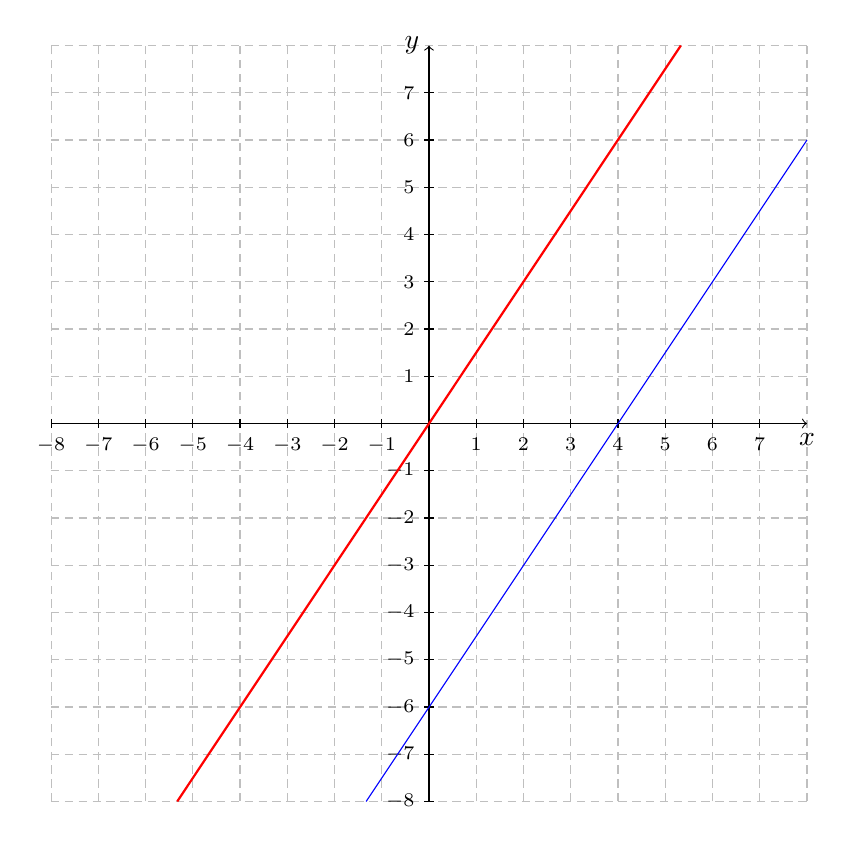
\begin{tikzpicture}[scale=0.6]
% grid
\draw [densely dashed, gray!50]    (-8,-8) grid (8,8);  
% ticks
\foreach \i in {-8,...,-1,1,2,...,7}
{
\draw (\i,0.1) -- ++ (0,-0.2) node[below,font=\scriptsize] {$\i$};
\draw (0.1,\i) -- ++ (-0.2,0) node[left, font=\scriptsize] {$\i$};
}
% axis
\draw [->] ( 0,-8) -- (0,8) node [left ] {$y$};
\draw [->] (-8, 0) -- (8,0) node [below] {$x$};
% graph
\draw [draw=red,thick] (-5.33,-8) -- (5.33,8);
\draw [draw=blue]   (-1.33,-8) -- (8,6);
\end{tikzpicture}





\end{document}
